\documentclass[a4paper,12pt,twoside]{article}

\usepackage{graphicx}
\usepackage{amsmath}
\setlength{\oddsidemargin}{-1.5cm}
\setlength{\evensidemargin}{-2.0cm }
\setlength{\textwidth}{18 cm}
\setlength{\textheight}{25cm}
\voffset=-2.5cm
%\author{Nigel Wilding}
\input epsf
\begin{document}
\pagestyle{empty}
%\input tcmjnl
\def\deg{^\circ}
\def\h{\hfil\break}
\def\hh{\h\h}
\def\singlespace{\baselineskip=\normalbaselineskip}
\singlespace\noindent
\centerline{\bf Mathematical Physics: Problems on Phase transitions: outline solutions}\\

%{\it Please hand in a written answer to question 2}

\begin{enumerate}

\item {\bf Existence of a phase transition in $d=2$.}

Consider the simplest elementary excitation that will destroy long range
order in the 2d system: a domain wall of $N$ segments which divides an Ising system of $L\times L$ spins into a spin up and a spin down part. 

\begin{figure}[h]
\centerline{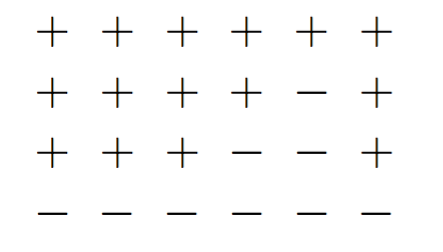
\includegraphics[width=6.5cm,clip=true]{Figs/domain}}
\caption{An $N$-step domain wall in an Ising lattice}
\end{figure}

The associated energy cost is $2JN \equiv \Delta E$. 

To evaluate the entropy gain due to a domain wall in the system we have to estimate $\Omega$ the number of possible paths for the domain wall.
If we start at the left hand side then there are $L$ starting positions.
At each step the domain wall can move to the right, move up or move down. This implies that the number of domain walls is approximately

$$
\Omega\approx L3^N
$$
Hence the entropy gain is:

$$
\Delta S=Nk_B\ln 3+k_B\ln L\approx Nk_B\ln 3  
$$

Accordingly, the change in the free energy associated with inserting such a domain wall into an ordered system is

\[
\Delta F=\Delta E-T\Delta S= N(2J-k_BT\ln 3)
\]

For small enough $T <2J/(k_B\ln 3)$, the free energy change is positive.
Thus the ordered phase is free energetically stable against formation of a
wall. Accordingly there will be a non zero value for $T_c$ in two dimensions.

\item {\bf Correlation Length}

Denote by $m$ the number of domain walls between sites $i$ and $j$. Then
$s_is_j=1$ for $m$ even, and $s_is_j=-1$ for $m$
odd.

Hence

\[
\langle s_i s_j\rangle =\sum_m p_m(-1)^m
\]
with $p_m$ the probability of finding $m$ domain walls between them.

Now $p_m$ is given by the binomial distribution, with the probability of
a single domain wall at each bond given by 

\[
p=\frac{e^{-2J/k_BT}}{1+e^{-2J/k_BT}}
\]
and the probability of no wall is $1-p$. 
Now, in the regime where $T$ is small, $p$ is very small, and there will be few domain walls between
sites $i$ and $j$. If additionally, $R_{ij}=|i-j|a$ is large, it tranpires that the binomial distribution
assumes the limiting form of a Poissonian distribution (revise this if necessary). Thus

\[
p_m=\frac{\bar{m}^me^{-\bar {m}}}{m!}
\] 

where $\bar{m}=p|j-i|=pR_{ij}/a$ . Then

\begin{eqnarray*}
\langle s_i s_j\rangle &=& e^{-\bar {m}}\sum_m\frac{(-1)^m\bar{m}^m} {m!}\approx e^{-2\bar{m}}\\
                       &=& e^{-2pR_{ij}/a}\\
                       &=& e^{-R_{ij}/\xi}
\end{eqnarray*}
with $\xi=a/2p$, the correlation length. 


\item{\bf A model fluid}

The van der Waals (vdW) equation of state (See Sec 4.4.1 of the book by
Yeomans) is essentially a mean field theory for fluids. It relates the
pressure and the volume of a fluid to the temperature:

\[
\left(P+\frac{a}{V^2}\right)(V-b)=Nk_BT
\]
where $a$ and $b$ are constants chosen to describe a specific substance and $N$ is Avogadro's number. Hence

\begin{equation}
P=\frac{Nk_BT}{V-b}-\frac{a}{V^2}
\label{eq:pres}
\end{equation}

\[
\Rightarrow \frac{\partial P}{\partial V}=\frac{-Nk_BT}{(V-b)^2}+\frac{2a}{V^3}
\]

\[
\Rightarrow \frac{\partial^2 P}{\partial V^2}=\frac{2Nk_BT}{(V-b)^3}-\frac{6a}{V^4}
\]

Now at criticality (ie. a continuous transition).

\[
\left(\frac{\partial P}{\partial V}\right)_T=\left(\frac{\partial^2 P}{\partial V^2}\right)_T=0
\]

Thus

\begin{eqnarray*}
\frac{Nk_BT}{(V_c-b)^2} &=& \frac{2a}{V_c^3}\\
\frac{2Nk_BT}{(V_c-b)^3} &=& \frac{6a}{V_c^4}
\end{eqnarray*}

solving for $V_c$ and $Nk_BT_c$ yields

\begin{eqnarray*}
V_c &=& 3b\\
Nk_BT_c &=& \frac{8a}{27b}
\end{eqnarray*}

Substituting these two results into eq.~\ref{eq:pres} yields 

\[
P_c=\frac{a}{27b^2}
\]

Now let $P=P_c p, V=V_cv, T=T_ct$ in the vdW eqn. (Note that in this
context $t$ is not the reduced temperature).

\[
\left(P_cp+\frac{a}{(V_cv)^2}\right)(V_cv-b)=N_Ak_BT_ct
\]

Substituting in for $V_c, N_Ak_BT_c$ and $P_c$

\begin{eqnarray*}
\left(p\frac{a}{27b^2}+\frac{a}{9b^2v^2}\right)\left(3bv-b\right)&=&\frac{8a}{27b}t\\
\Rightarrow\left(p+\frac{3}{v^2}\right)\left(v-\frac{1}{3}\right)&=&\frac{8}{3}t\\
\end{eqnarray*}
This expression for the equation of state in terms of reduced variables
is useful because reference to the system specific parameters $a$ and
$b$ has vanished. In this form the equation is therefore universal. 

Plotting $P/P_c$ vs $V/V_c$ for isotherms (values of $t$) and focussing
on the region close to the critical point, one finds

\begin{figure}[h]
\centerline{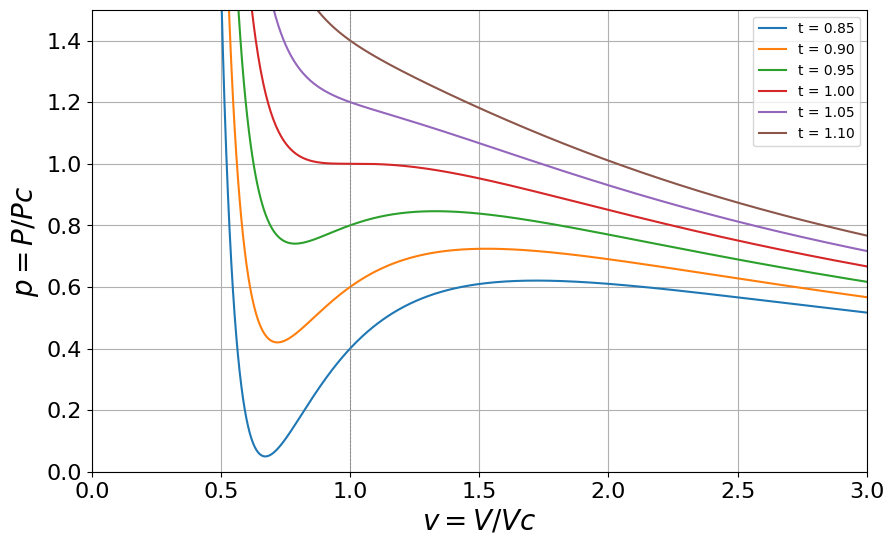
\includegraphics[width=11.0cm,clip=true]{Figs/VdW_isotherms}}
\caption{Isotherms of $p$ vs $v$ for various $t$.}
\end{figure}


\begin{figure}[h]
\centerline{\includegraphics[width=6.5cm,clip=true]{Figs/dp}\includegraphics[width=6.5cm,clip=true]{Figs/dpp}}
\caption{(left) $\frac{\partial p}{\partial v}$ for $T=T_c$.
(right) $\frac{\partial^2 p}{\partial v^2}$ for $T=T_c$.}
\end{figure}

Plotting $(\frac{\partial p}{\partial v})_{t=1}$ and $(\frac{\partial^2 p}{\partial
v^2})_{t=1}$, we see that there is indeed a point of inflexion on the
critical isotherm, at $v=1$, this is the critical point (ie. a continuous
phase transition).

Subcritical isotherms (first order phase transition) exhibit a so called
van-der Waals loop. 

To find the compressibility critical exponent $\gamma$, we recall that

\[
\kappa_T=\frac{-1}{V}\left(\frac{\partial V}{\partial P}\right)_T=\frac{-1}{p_cv}\left(\frac{\partial v}{\partial p}\right)_t\propto \tilde{t}^{-\gamma}
\]
with $\tilde{t}=(T-T_c)/T_c$ small.

Now from the reduced equation of state

\[
\frac{\partial p}{\partial v}=\frac{-8t}{3(v-1/3)^2}+\frac{6}{v^3}
\]
setting $t=\tilde{t}+1$ and $v=1$ gives $\frac{\partial p}{\partial v} =-6\tilde{t}$, ie the
compressibility diverges 

\[
\kappa_T\propto \tilde{t}^{-1}
\]
ie. $\gamma=1$, which is the same as the mean field result which we
derived in another context of the magnetic susceptibility.

\item {\bf Mean field theory of the Ising model heat capacity}

We insert into the expression for the mean Ising energy

\[
\langle E \rangle =-J\sum_{<i,j>}\langle s_is_j\rangle\:, 
\]
the simplest mean field approximation $\langle s_is_j\rangle=\langle s_i\rangle\langle s_j\rangle=m^2$.
Recalling the behaviour of the order parameter for small $t$, that 
the number of bonds $=qN/2$, and the mean field value
of $T_c=qJ/k_B$, we have for $T<T_c$

\begin{eqnarray*}
\langle E \rangle &=& \frac{-NqJm^2}{2}\\
\:                &=& \frac{3NqJt}{2}\\
\:                &=& \frac{3Nk_B(T-T_c)}{2}\\
\end{eqnarray*}
while $\langle E \rangle= {\rm constant}$ for $T>T_c$.

Hence differentiating, we find

\begin{eqnarray*}
C_H&=& 0 \hspace*{20mm} T>T_c\\
C_H&=& 3Nk_B/2 \hspace*{6mm} T\le T_c
\end{eqnarray*}

This independence of the heat capacity on $t$ corresponds to a critical
exponent $\alpha=0$

\item {\bf Magnetisation and fluctuations}

The free energy is 

\[
F=-k_BT\ln Z
\]
with the partition function 

\[
Z=\sum_{\{s\}}\exp[-({\cal H}-hM)/k_BT]
\]

Thus

\begin{eqnarray*}
-\left(\frac{\partial F}{\partial h}\right)_T &=& k_BT\frac{1}{Z}\left(\frac{\partial Z}{\partial h}\right)_T\\
\: &=&\frac{1}{Z}\sum_{\{s\}}M \exp[-({\cal H}-hM)/k_BT]\\
   &=& \langle M\rangle
\end{eqnarray*}
where we have used the definition of the average of an observable given
in lectures.

Now 
\begin{eqnarray*}
\left(\frac{\partial^2 F}{\partial h^2}\right)_T &=& -k_BT\left[\frac{1}{Z}\left(\frac{\partial^2 Z}{\partial h^2}\right)_T-\left(\frac{\partial Z}{\partial h}\right)_T\frac{1}{Z^2}\left(\frac{\partial Z}{\partial h}\right)_T\right]\\
\: &=&\frac{-1}{k_BT}\left[\frac{1}{Z}\sum_{\{s\}}M^2 \exp[-({\cal H}-hM)/k_BT]-\langle M\rangle^2\right]\\
\:   &=& \frac{-1}{k_BT}\left[\langle M^2\rangle-\langle M\rangle^2\right]
\end{eqnarray*}
You should recognise the terms in square brackets as the variance of the
magnetisation distribution.

Thus the susceptibility is 
\[
\chi_H\equiv\frac{\partial \langle M\rangle}{\partial h}=\frac{1}{k_BT}\left[\langle M^2\rangle-\langle M\rangle^2\right]
\]

Incidently, this is known as the fluctuation-dissipation theorem. It is
a neat result, because it allows you to calculate the response to a
perturbation from equilibrium, without actually perturbing the system!
Instead one merely looks at the form of the equilibrium fluctuations. It is used extensively in computer simulations.

\item {\bf Spin-1 Ising model}

As in lectures, the mean field Hamiltonian for a single spin is 

\[
{\cal H}(s_0)=-s_0\left(qJm + H\right)
\]
The probability of finding this spin with value $s_0$ is

\begin{eqnarray*}
p(s_0) &=& \frac{e^{-\beta{\cal H}(s_0)}} {\sum_{s_0=0,\pm 1}e^{-\beta{\cal H}(s_0))}}\\
&=&\frac{e^{\beta s_0(qJm+H)}}{1+e^{\beta(qJm+H)}+e^{-\beta(qJm+H)}}
\end{eqnarray*}

Now for consistency $\langle s_0\rangle=m$, so

\begin{eqnarray*}
m &=& \sum_{s_0=0,\pm 1}s_0p(s_0)\nonumber\\
 \:&=& \frac{0+e^{\beta(qJm+H)}-e^{\beta(qJm+H)}} {e^0+e^{\beta(qJm+H)}+e^{-\beta(qJm+H)}}\\
 \:&=&  \frac{2\sinh[\beta(Jqm+h)]}{1+2\cosh[\beta(Jqm+h)]}\\
\end{eqnarray*}

To get the critical temperature, we can solve this graphically. One plots
the RHS as a function of $m$, for various $\beta$. On the same graph one
plots the curve $y=m$ (representing the LHS). $T_c$ is the highest $T$ for which
the two curves intersect.

\item{\bf Transfer Matrix}

The transfer matrix is a list of the possible interactions of a pair
of spins with one another and with a magnetic field. For a 1d spin-1/2
system it takes the form:

\begin{equation}
{\bf V}(H)=\left(
\begin{array}{cc}
e^{\beta(J+H)} & e^{-\beta J} \\
e^{-\beta J}   & e^{\beta(J-H)}
\end{array} \right)
\end{equation}

We need to find the eigenvalues, so we solve
the characteristic equation det(${\bf V}-\lambda {\bf I})=0$, i.e.

\[
{\bf V}(H)=\left|
\begin{array}{cc}
e^{\beta(J+H)} -\lambda & e^{-\beta J} \\
e^{-\beta J}   & e^{\beta(J-H)}-\lambda
\end{array} \right| =0
\]

Then $\lambda^2-(a+d)\lambda+(ad-bc)=0$. So

\begin{eqnarray*}
\lambda_\pm &=& \frac{a+d\pm\sqrt{(a+d)^2-4(ad-bc)}}{2}\\
\lambda_{\pm} &=& e^{\beta J}\cosh(\beta H) \pm \frac{1}{2}\sqrt{e^{2\beta J}4\cosh^2\beta H-4(e^{2\beta J}-e^{-2\beta J})}\\
\lambda_{\pm} &=& e^{\beta J}\cosh(\beta H) \pm \sqrt{e^{2\beta J}\sinh^2\beta H+e^{-2\beta J}}.
\end{eqnarray*}
(You'll need the identity  $\cosh^2 x-\sinh^2 x = 1$).

From lectures, you should know that the partition function
\begin{eqnarray*}
Z={\rm Tr}({\bf V}^N)&=&\lambda_+^N+\lambda_-^N\\
&\approx & \lambda_+^N \hspace{5mm}{\rm N~large}
\end{eqnarray*}
where $\lambda_+$ is the largest of the two evals.

Hence the free energy $F=-k_BT\ln(Z)$ can be written 

\[
F=-Nk_BT\ln \left[e^{\beta J}\cosh(\beta H) + \sqrt{e^{2\beta J}\sinh^2\beta H+e^{-2\beta J}}\right].
\]

Now the magnetisation per site is 

\[
m=-\frac{1}{N}\frac{\partial F}{\partial H}=\frac{k_BT}{\lambda_+}\frac{\partial \lambda_+}{\partial H}
\]

You can either be a hero here, or use Maple or Mathematica. I did the latter to find
the stated result.

\[
m=\frac{\sinh \beta H}{\sqrt{\sinh^2\beta H+\exp{(-4\beta J)}}}
\]

Hence at zero $H$, there is no spontaneous magnetisation at any $T$.

\item {\bf Lattice gas model}
The aim is to show that the Lattice Gas Hamiltonian is isomorphic to that of the Ising model.

Substituting $c_i=(1+s_i)/2$, $c_j=(1+s_j)/2$ into the Lattice Gas
Hamiltonian
\begin{equation}
{\cal H}_{LG}=-\epsilon\sum_{<i,j>}c_ic_j -\mu\sum_ic_i
\end{equation}

yields

\begin{eqnarray*}
{\cal H}_{LG}&=&\frac{-\epsilon}{4}\sum_{<i,j>}(s_is_j+s_i+s_j+1)-\frac{\mu}{2}\sum_i(1+s_i)\\
           &=&\frac{-\epsilon}{4}\sum_{<i,j>}s_is_j-\frac{q\epsilon}{4}\sum_i s_i-\frac{\mu}{2}\sum_is_i +{\rm constants}\\
\end{eqnarray*}
where the additive constants are configuration independent. Note here
that a sum over bonds $\sum_{<i,j>}$ is equal to $q/2$ times a sum over $\sum_i$, because
there are $Nq/2$ bonds on the lattice, and hence $q/2$ bonds per site.

Comparison with the Ising model Hamiltonian 
\[
{\cal H}_I=-J\sum_{\langle i,j\rangle}s_is_i-h\sum_i s_i
\]
 leads to the mapping

\[
J=\frac{\epsilon}{4}, \hspace*{1cm} h=\frac{(q\epsilon+2\mu)}{4}
\]

Note one can also use the transformation $c_i=(1-s_i)/2$, which simply leads to different signs in the mapping.

\item {\bf Landau theory}

If this were an Ising model problem (ie a microscopic model) we could
write down the partition function, get an explicit expression for the
free energy and differentiate once (wrt $T$) to get the energy and again
(wrt $T$) to get the heat capacity. But the
starting point for Landau theory is the free energy itself, so we need
another starting point, namely thermodynamics. The appropriate
thermodynamic potential for the magnet is $F=U-TS-MH$ with $U$ the internal
energy. Then 

\begin{eqnarray*}
dF &=& dU-TdS-SdT-MdH-HdM\\
\: &=& TdS+HdM-TdS-SdT-MdH-HdM\\
\: &=& -SdT-MdH\\
\end{eqnarray*}
where we have used the first law for a magnet $dU=TdS+HdM$, 

Thus
\begin{eqnarray*}
\left(\frac{\partial F}{\partial T}\right)_H&=&-S\\
-T\left(\frac{\partial^2 F}{\partial T^2}\right)_H&=&T\frac{dS}{dT}=\frac{dQ}{dT}\\
C_H=-T\left(\frac{\partial^2 F}{\partial T^2}\right)_H
\end{eqnarray*}
where $C_H$ is the specific heat at constant field and we have used the
fact that $dS=dQ/T$.

Now from lectures, the equilibrium magnetisation in the Landau free
energy is given by 

\[
m^2=\frac{-a_2}{2a_4}
\]
for $T<T_c$ and zero otherwise. Substituting this into the Landau free energy
$F=F_0+a_2m^2+a_4m^4$ gives

\begin{eqnarray*}
F = F_0 \hspace*{1cm} T>T_c\nonumber\\
F = -a_2^2/4a_4 \hspace*{1cm} T < T_c
\end{eqnarray*}
Using the fact that $a_2=\tilde{a_2} t$, with $t=(T-T_c)/T_c$ and differentiating wrt $T$
twice, to get the heat capacity, we find 

\begin{eqnarray}
C_H &=& 0 \hspace*{1cm} T\to T_c^+\nonumber\\
C_H &=& \frac{T\tilde a_2^2}{2a_4T_c^2} \hspace*{1cm} T \to T_c^-\:,
\end{eqnarray}

The jump discontinuity rather that a divergence in the specific heat at
$T=T_c$ formally corresponds to a critical exponent $\alpha=0$.

To get the susceptibility exponent, we add a magnetic field to the free
energy


\[
F(m)=F_0+a_2m^2+a_4m^4-Hm
\]

Then the equilibrium magnetisation satisfies

\begin{eqnarray*}
\frac{dF}{dm}&=&2\tilde{a_2} tm+4a_4m^3-H=0\\
\Rightarrow H&=&2\tilde{a_2} tm+4a_4m^3\\
\Rightarrow \left(\frac{\partial H}{\partial m}\right )_T&=&2\tilde{a_2} t+12a_4m^2\\
\end{eqnarray*}

Now using the results that $m^2=0$ for $t>0$ and $m^2=-\tilde{a_2}t/(2a_4)$ for $t<0$, we have 
that in both cases 

\[
\left(\frac{\partial H}{\partial m}\right )_T\propto t\\
\]

Hence

\[
\left(\frac{\partial m}{\partial H}\right )_T\propto t^{-1}
\]
so $\gamma=1$.


\item {\bf Scaling laws}

First of all recall the definition of the critical exponents: 

\begin{eqnarray*}
m      & \propto & t^{\beta};\hspace*{6mm}(h=0)\\ 
\chi_T & \propto & t^{-\gamma};\hspace*{6mm}(h=0)\\ 
C_H & \propto & t^{-\alpha};\hspace*{6mm}(h=0)\\ 
m & \propto & h^{1/\delta}.\hspace*{6mm}(t=0)\\ 
\end{eqnarray*}
The free energy in generalised homogeneous form is 

\[
F(\lambda^a t,\lambda^b h)=\lambda F(t,h) 
\]

The first of the scaling relations to be derived was covered in lectures:
Let $\lambda^a=1/t$, so that $\lambda=t^{-1/a}$. Then

\begin{eqnarray*}
F(t,h)&=&t^{1/a}F(1,t^{-b/a}h)\\
m(t,h)&=&-\left(\frac{\partial F}{\partial h}\right)_t= -t^{(1-b)/a} \left.\frac{\partial F(1,y)}{\partial y}\right|_{ht^{-b/a}}=t^{(1-b)/a}m(1,ht^{-b/a})\\
\end{eqnarray*}
so when $h=0$, we have $m(1,t^{-b/a}h)=m(1,0)={\rm const}$ and hence we can identify
$\boxed{\beta=(1-b)/a}$.

We also have for the isothermal susceptibility

\[
\chi=\left(\frac{\partial m}{\partial
h}\right)_t=-t^{(1-2b)/a}\left.\frac{\partial^2 F(1,y)}{\partial y^2}\right|_{ht^{-b/a}},
\]
so taking again $h=0$, we find $\boxed{\gamma=(2b-1)/a}$.

For the specific heat at constant (zero) field, we have the definition:
\[
C_H = \left(\frac{\partial E}{\partial T}\right)_{h=0}=-T\left(\frac{\partial^2F}{\partial T^2}\right)_{h=0}\:,
\]
where in the last step have used $E=-\partial (\beta F)/\partial\beta$, with $\beta=(k_BT)^{-1}$ (see fig 3). Alternatively one can use the thermodynamic derivation of this relation given in an earlier problem on Landau theory. Transforming from $T$ to $t=(T-T_c)/T_c$ and inserting the generalised homogeneous form for $F$ gives:

\begin{eqnarray*}
C_H &=& -\frac{T}{T_c^2}\frac{\partial^2}{\partial t^2}[t^{1/a}F(1,t^{-b/a}h)]\\
C_H &\approx& -\frac{1}{T_c}\frac{\partial^2}{\partial t^2}[t^{1/a}F(1,t^{-b/a}h)]\\
C_H &=& -\frac{1}{T_c}\frac{1}{a}(\frac{1}{a}-1)t^{(1/a-2)}F(1,0)\\
\end{eqnarray*}
Here we have neglected all derivatives of $F$ since they are multiplied
by at least one power of $h$ which is zero. Hence $\boxed{\alpha=2-1/a}$.

Finally, if we let $\lambda^b=1/h$, so that $\lambda=h^{-1/b}$ and
consider the critical isotherm $t=0$. Then

\begin{eqnarray*}
F(t,h)&=&h^{1/b}F(h^{-a/b}t,1)\\
\Rightarrow m(t,h)&=& \frac{ta}{b}h^{(1-a-b)/b}\left.\frac{\partial F(x,1)}{\partial x}\right|_{h^{-a/b}t}-\frac{1}{b}h^{1/b-1}F(h^{-a/b}t,1).
\end{eqnarray*}
so when $t=0$, we get $m(0,h)$ and can identify $\boxed{\delta=b/(1-b)}$.

To derive the relationships (``scaling laws'') among the critical exponents, we eliminate $a$ and $b$ from the boxed scaling relations. 
Setting $a=(2-\alpha)^{-1}$ in the first scaling relation, we
find $b=1-\beta/(2-\alpha)$. Substituting this into the second scaling
relation gives the second of the two scaling laws quoted in the notes. Substituting
into the 4th scaling relation gives the first scaling law.
\item {\bf Renormalization transformation for the 1D Ising model}

Start by drawing a diagram!

\begin{figure}[h]
\centerline{\includegraphics[width=10.0cm,clip=true]{Figs/1DIsing}}
\caption{Renormalization of the 1D Ising model by a scale factor $b=2$.
(a) the original lattice, (b) renormalized lattice, (c) the
renormalized lattice with the spins re-numbered consecutively.}
\end{figure}

\begin{itemize}

\item[(a)] As argued in the section of the notes on the transfer
matrix, the partition function can be written as the configurational
sum over a product of exponential factors, each of which depends only
on one of the even numbered spins.

\[
Z=\sum_{s}\prod_{i=2,4,6...} [\exp [Ks_i(s_{i-1}+s_{i+1})+2C]
\]

Now the even numbered spins do not interact with one another. Thus we
can perform the partial sum over the two possible values of $s_i$,
gives immediately

\[
Z=\sum_{s_1,s_3,s_5...}\prod_{i=2,4,6...} [\exp
[K(s_{i-1}+s_{i+1})+2C] + \exp[-K(s_{i-1}+s_{i+1})+2C]
\]

\item[(b)] Relabeling (with a new dummy index $j$) the surviving odd spins so that they are numbered
consecutively gives

\[
Z=\sum_{\{s\}}\prod_{j=1}^{N/2}[\exp [K(s_j+s_{j+1})+2C] + \exp[-K(s_j+s_{j+1})+2C]\:,
\]

To make the renormalisation iterable, we now demand that this partially
summed partition function has the same functional form as that of an
Ising lattice of $N/2$ spins, ie. that it has the form

\[
Z^\prime=\sum_{\{s\}}\prod_{j=1}^{N/2}\exp[K^\prime s_js_{j+1}+C^\prime]\:,
\]
for all $s_j,s_{j+1}=\pm 1$.

By inspection, the two partition function are equivalent for the two
respective distinct cases $s_j=s_{j+1}$ and $s_j=-s_{j+1}$ provided that

\begin{eqnarray*}
\exp(K^\prime+C^\prime) &=& \exp(2C)[\exp(2K)+\exp(-2K)] \\
\exp(-K^\prime+C^\prime) &=& 2\exp(2C).
\end{eqnarray*}

These two equations express the two unknown renormalised quantities $K^\prime$ and
$C^\prime$ in terms of the original quantities $K$ and $C$.

\item[(c)] 

Solving for $K^\prime$ gives

\[
K^\prime = (1/2)\ln (\cosh 2K) 
\]

Sticking in some numbers should convince you that $K^\prime < K$, so the
RG transformation drive the effective coupling to the high
temperature fixed point. This makes sense because the renormalisation
reduces the effective correlation length.

\item[(d)] 

Comparing factors in the product of exponentials appearing in the expressions for
$Z$ and $Z^\prime$, we have

\[
\exp [K(s_j+s_{j+1})+2C] + \exp[-K(s_j+s_{j+1})+2C]=\exp[K^\prime s_js_{j+1}+C^\prime]
\]

Thus

\[
\exp [K(s_j+s_{j+1})] + \exp[-K(s_j+s_{j+1})]=\exp[K^\prime s_js_{j+1}]\exp[C^\prime-2C]
\]

Now noting from the previous part of the question, that
$\exp(C^\prime-2C)=2\exp(K^\prime)$, it follows that the partition
functions of an Ising model $Z(K,N)$ is related to that of a renormalised
Ising model $Z(K^\prime,N/2)$ by 

\[
Z(K,N)=2^{N/2}\exp(NK^\prime/2)Z(K^\prime,N/2)
\]

\end{itemize}

\item {\bf Iterating an RG transformation for the free energy}

This transformation is the inverse of that arising from decimation, so if we start with $K^\prime$ we generate $K$.
Choose as a start value $K^\prime=0.01$ and $\beta f(K^\prime)\approx -\ln 2$. Then we iterate the equations:

\begin{eqnarray*}
K &=& (1/2)\cosh^{-1}(\exp 2K^\prime) \\
\beta f(K) &=& (1/2)\beta f(K^\prime)-(1/2)\ln 2-K^\prime/2\\
\end{eqnarray*}

This gives 

\begin{eqnarray*}
K &=& 0.100334\\
\beta f(K) &=& -0.698147
\end{eqnarray*}

We now use these numbers as the new $K^\prime$ quantities, and obtain

\begin{eqnarray*}
K &=& 0.327447\\
\beta f(K) &=& -0.745814
\end{eqnarray*}
and so on.

Here is the result:

%\begin{table}[h]
\begin{tabular}{lccc}
Iteration  r & K & RG & Exact\\\hline
 & 0.01     & $-\ln 2$ & -0.693197\\
1 & 0.100334 & -0.698147 & -0.698172\\
2 & 0.327447 & -0.745814 & -0.745827\\
3 & 0.636247 & -0.883204 & -0.883210 \\
4 & 0.972710 & -1.106229 & -1.106302 \\
5 & 1.316710 & -1.386078 & -1.386080 \\
6 & 1.662637 & -1.697968 & -1.697968 \\
7 & 2.009049 & -2.026876 & -2.026877 \\
8 & 2.355582 & -2.364536 & -2.364537 \\
\end{tabular}
%\end{table}

\end{enumerate}
Notice how the results approach the correct low temperature limit $\beta f=-K$.

\end{document}

